\documentclass[12pt,a4paper]{extarticle}

\usepackage{extsizes}	
\usepackage[english,russian]{babel}
\usepackage[utf8]{inputenc}
\usepackage{verbatim}
\usepackage{algorithm}
\usepackage{clrscode}
\usepackage{varwidth}
\usepackage{xcolor}
\usepackage[final]{graphicx}
\usepackage{amsmath, amssymb}
\usepackage{amsthm}
\usepackage[left=30mm,right=15mm,top=20mm,bottom=25mm]{geometry}
\usepackage{setspace}
\onehalfspacing

\usepackage{amsmath, amssymb}
\usepackage{amsthm}
\usepackage{enumerate}
\usepackage{hyperref}
\usepackage{setspace}
\setstretch{1.15}
\setcounter{page}{2}

\usepackage{geometry}
\geometry{top=2cm}
\geometry{bottom=2.5cm}
\geometry{left=3cm}
\geometry{right=2cm}

\begin{document}

\tableofcontents
\newpage
\section{Введение}

C ростом доступности и мощности компьютеров растет интерес к практическим исследованиям в различных областях науки. Так, в последние годы набирают популярность исследования по анализу и обработки больших объемов данных. Результаты, полученные в этой области, способствовали запуску нескольких крупно-масштабных проектов: предсказание в изменениях климата, моделирование формирования галактик и биомолекулярное моделирование[2].


Несмотря на столь стремительный рост практический исследований, не существует четких стандартов и требований, предъявляемых к публикации их результатов. Хотя создание воспроизводимых результатов является главной целью научных исследований, ведь воспроизводимые результаты позволяют каждому новому поколению ученых строить свои исследования на результатах предыдущего поколения, сейчас достаточно трудно, а порой и вовсе невозможно воспроизвести практические результаты, которые ученые представляют на конференциях и описывают в своих исследованиях.


В исследовании G. Robles[1] освещает данную проблему применительно к области анализа и обработки данных. Им была исследована 171 статья на предмет их не реальной, а потенциальной воспроизводимости. В исследовании было выделено несколько критериев оценки: доступность исходных данных, доступность ``обработанных'' данных и доступность инструментов, с помощью которых проводились исследования. На диаграмме изображено типичное исследование в области анализа и обработки данных:


\begin{figure}[h]
    \begin{center}
        \begin{picture}(70,90)(90,0)
        	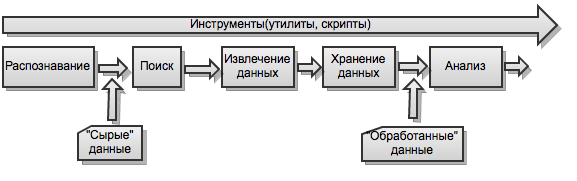
\includegraphics[scale=0.5]{research.png}
        \end{picture}
    \end{center}
    \caption{Структура типичного исследования в области анализа и обработки данных}
    \label{typical_research}
\end{figure}


На этой диаграмме видно, какое место занимают в исследовании в области обработки
данных исходные данные, ``обработанные'' данные и инструменты.


В исследовании G.Roubles было сделано несколько выводов:
\begin{itemize}
	\item Исходные данные доступны в более чем 75 \% исследований.
	\item ``Обработанные'' данные практически недоступны. Хотя, они чрезвычайно важны для повторяемости исследования. Более того, практически никто из исследователей не пытался использовать в своей работе ``обработанные'' данные, предпочитая использовать исходные данные.
	\item В более, чем половине статей не предоставляются данные о используемых инструментах.  Также данные о чуть менее, чем четверти инструментов доступны, но без указания версий и других сведений, которые важны для воспроизводимости исследований.
\end{itemize}


Хотя его исследования и затрагивают лишь “потенциальную” воспроизводимость и лишь область анализа и обработки данных(как нам кажется, в других областях все обстоит схожим образом), выводы неутешительные: половину исследований даже потенциально невозможно воспроизвести.


В связи с этим, остро встает вопрос о том, что необходимо предпринять для того, чтобы улучшишь воспроизводимость исследований. В своем исследовании G. Roubles выдвигает некоторые идеи, которые могут помочь в этом:

\begin{itemize}
	\item Доступность исходных данных недостаточна. Необходимо четко и полно описывать, какие данные вы использовали. Если вы выбираете 100 случайных проектов с Sourceforge(\url{http://sourceforge.net}), то укажите, какие именно проекты вы выбрали. В дополнение к этому, необходимо указывать версии данных или их временную метку. Также необходимо указывать версии используемых инструментов и предоставить возможность для их загрузки.
	\item Системный подход: выделить специальную секцию в статье, где будет предоставлена вся необходимая информация об исследовании и его воспроизводимости.
	\item Создание инфраструктуры. Инфраструктура предлагала бы возможность предоставлять и обращаться к данным и инструментам и легко их переиспользовать и улучшать.
\end{itemize}


Несмотря на то, что вышеописанные идеи выдвинуты применительно к исследованиям в области обработки данных, их можно применять и в любых практических исследованиях. 


В связи с тем, что наша группа занимается практическими исследованиями в области сжатия и обработки данных, перед нами встала задача воспроизводимости наших исследований. Далее в работе представлено концептуальное решение, основанное на идеях G. Roubles, а также, в некотором приближении, его реализация.

\newpage

\section{Требования}
На наш взгляд, решением задачи воспроизводимости наших исследований должна стать инфраструктура, удовлетворяющая некоторые требования.
Исходя из этого, мы определили основные требования к создаваемой инфраструктуре:

\subsection{Управление данными и исследованиями.}
Основываясь на специфике наших исследований, можно выделить две основные сущности, вокруг которых необходимо строить использование инфраструктуры: данные и исследования(в последние входят, например, алгоритмы сжатия). Нами выделено несколько основных сценариев использования инфраструктуры:
\begin{itemize}
	\item{Запуск исследований на новых данных.} Инфраструктура должна давать возможность загрузки файла и запуска выполнения на нем наших исследований. Исходя из специфики исследований, а именно больших объемов данных, процессы загрузки и выполнения могут занимать достаточно длительное время. В связи с этим, прогресс по данным процессам должен быть наглядно представлен. 
	\item{Перезапуск исследований.} В связи с улучшением или исправлением ошибок в наших исследованиях, инфраструктура должна давать возможность перезапустить их выполнение.
	\item{Работы с результатами исследований.} Необходимо реализовать механизмы сравнения результатов исследований по различным характеристикам(скорость работы, размер сжатого представления, потребление памяти и т.д.). Также необходимо предоставить механизмы для экспорта из инфраструктуры результатов исследований: не только характеристики, но и сами сжатые представления. 
\end{itemize}

\subsection{Общедоступность результатов исследований и исходных данных.} 
Исследования могут занимать существенное время, поэтому результаты должны быть общедоступны. Под результатами здесь мы понимаем не только некоторую статистику по производительности, объему потребляемой памяти и некоторым другим параметрам, но также и результаты работы самих алгоритмов сжатия(в нашем случае это сжатое представление данных). Более того, должны быть доступны и исходные данные. В отличие от сжатых представлений, которые имеют сравнительно небольшой объем, исходные данные имеют намного больший объем, который может доходить до нескольких десятков гигабайт, что затрудняет возможность сделать их общедоступными.


\subsection{Общедоступность исходного кода} Исходный код инфраструктуры должен располагаться в публичном репозитории контроля версий для того, чтобы у любого исследователя была возможность воспроизвести наши исследования.

\subsection{Простота сборки и запуска.}  В данный момент, неподготовленному исследователю будет очень трудно собрать(скомпилировать) исходных код нашего проекта, провести на нем аналогичные исследования и независимо получить аналогичный результат. В связи с этим возникает потребность в простой сборке и простом запуске инфраструктуры.

\subsection{Кроссплатформенность.} По статистике от компании Net Applications, на апрель 2012 года имеет место следующее распределение операционных систем в мире:

\begin{figure}[h]
    \begin{center}
        \begin{picture}(70,90)(90,0)
        	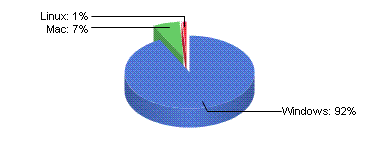
\includegraphics[scale=0.5]{os.png}
        \end{picture}
    \end{center}
    \caption{Мировое распределение операционных системы.}
    \label{typical_research}
\end{figure}


На графике мы видим, что на 8 \% компьютерах установлена не Microsoft Windows. Как нам кажется, это достаточно серьезная цифра, чтобы о ней стоило задуматься, тем более, что в рамках прикладных областей компьютерных наук, этот процент будет выше. В следствие этого, хотелось бы иметь инфраструктуру, которую было бы возможно  запустить на практически любом из компьютеров.

\subsection{Чистота исследований.} 
Необходимо обеспечить чистоту проведения исследований. Под чистотой мы понимаем следующее: часть инфраструктуры, которая запускает исследования, должна быть ограничена от все остальной инфраструктуры, чтобы исключить возможное воздействия остальных ее компонентов на результаты исследования.

\subsection{Масштабируемость.}
В контексте наших исследований возникает необходимость хорошей масштабируемости нашей инфраструктуры. Под хорошей мы понимаем горизонтальную масштабируемость. 


\newpage

\section{Концепция решения}
Первоначально нам необходимо понять, что будет представлять из себя инфраструктура. Существует два основных подхода: веб-приложение(Web Application) и настольное приложение(Desktop Application). В статье[3] Vinny Lingham выделяет 20 наиболее значимых причин, почему веб-приложение лучше настольного. Вот некоторые из них:
\begin{itemize}
	\item Не требует установки. Для начала работы с веб-приложением нужен лишь браузер.
	\item Прозрачное обновление. Все обновления происходят на сервере.
	\item Доступно всегда и везде. 
	\item Кроссплатформенность. Используется браузер(практически все современные браузеры портированы на большинство существующих платформ), что избавляет от необходимости реализовывать поддержку всех популярных платформ.
	\item Менее подвержено ошибкам, которые связаны с программно-аппаратными настройками операционной системы.
\end{itemize}

Также, исходя из этих вышеизложенных требований к инфраструктуре, настольное приложение нам не подходит по следующим причинам:
\begin{itemize}
	\item Плохая масштабируемость. Мы ограничены ресурсами одно лишь компьютера.
	\item Проблемы с чистотой исследования. На компьютере исследователя может стоять программное обеспечение, которое повлияет на результаты исследования(например, антивирус).
	\item Для решения проблемы общедоступности результатов исследований и исходных данных было бы необходимо искать сторонний сервис или же  делать свой. В веб-приложении данная проблема решается автоматически.
\end{itemize}

В результате, основой для нашей инфраструктуры было решено выбрать веб-приложение. Однако, запускать наши исследования непосредственно на веб-сервере нельзя, так как это вызывает все теже проблемы с чистотой исследования и масштабируемостью. Решением данной проблемы является использование сервис-ориентированной архитектуры при реализации инфраструктуры.

Сервис-ориентированная архитектура — это модульный подход к разработке программного обеспечения, основанный на использовании распределённых, слабо связанных заменяемых компонентов, оснащённых стандартизированными интерфейсами для взаимодействия по стандартизированным протоколам. Использование этой архитектуры способствует масштабируемости и управляемости создаваемой системы.	

Также стоит отметить, что очень важно реализовать инфраструктуру так, чтобы исследователь мог ее запустить даже на локальной машине, поэтому нам важна кроссплатформенность инфраструктуры в целом, а не только веб-приложения.

\subsection{Сервисы}
Сервисы по функциональности можно разделить на следующие типы:
\begin{itemize}
	\item Хранение данных
	\item Выполнение исследований
	\item Публикация результатов.
\end{itemize}

\subsubsection{Сервисы выполнения исследований}

При концептуальном осмыслении основных сценариев работы инфраструктуры, в частности, сценариев ``Запуска исследования на новых данных'' и 
``Перезапуска исследования'', возникает такое понятия как задача. Задача - некоторая собирательная абстракция, в которой собираются данные том, какое исследование и на каких данных необходимо запустить. Опишем жизненный цикл задачи:
\begin{itemize}
	\item Создание задачи.
	\item Выполнение задачи.
\end{itemize}

\paragraph{Создание задачи}
Для реализации данной части жизненного цикла задачи используется веб-приложение, в котором предоставляется удобный интерфейс для ее создания. Подробнее останавливаться на этом мы не будем, так как это не представляет особой сложности.

\paragraph{Выполнение задачи}
После того, как задача создана, она должны быть некоторым образом выполнена. Для реализации данного процесса необходимо два вида сервисов(мы полагаем, что сервис управления задачами один, а сервисов выполнения задачами - много):
\begin{itemize}
	\item Сервис выполнения задачи - занимается запуском реализованных в нем алгоритмов сжатия данных. 
	\item Сервис управления задачами - занимается распределением задач между сервисами их выполнения.
\end{itemize}
Дальше, для краткости, сервис управления задачами мы будет называть сервисом управления, а сервис выполнения задач - сервисом выполнения.

Работу сервиса управления и сервисов выполнения можно описать следующими процессами: 
\begin{itemize}
	\item Сервис выполнения обращается к сервису управления для получения очередной задачи. Сервис управления выбирает очередную активную задачу из хранилища задач, выдает задачу сервису выполнения и помечает ее как выполняемую им, внося соответстующие изменения в хранилище задач.
	\item При выполнении полученной задачи, сервис выполнения через фиксированные промежутки времени должен обращаться к сервису управления за продление ``ренты'' на задачу. Сервис управления при продлении ``ренты'' сервисом выполнения вносит соответстующие изменения в хранилище задач.
	\item Все задачи с непродленной ``рентой'' сервис управления задачами перестает считать выполняемыми и вновь делает их доступными для выполнения(внося соответствующие изменения в хранилище задач).
	\item В случае, если сервис выполнения(для определенности, назовем его сервисом 1) пытается продлить ``ренту'' на задачу, которая уже выдана другому сервису выполнения или вовсе недоступна, сервис управления останавливает выполнение задачи на сервисе 1. После этого сервис 1 обращается к сервису управления для получения очередной задачи.
	\item В случае успешного выполнения задачи сервисом выполнения, он записывает результаты в хранилище результатов и сообщает сервису управления об успешном выполнении задачи. Сервис управления вносит соответствующии изменения в хранилище задач.
\end{itemize}

Исходя из описания процессов работы сервиса управления задачами, даже в случае сбоя данного сервиса мы не можем потерять задачи, так как данный сервис не хранит в себе состояний задачи и сразу записывает все изменения в хранилище задач. Благодаря этому, в случае сбоя, заново запустив данный сервис, который при запуске прочитает данные из хранилища задач, мы вновь получим консистентное состояние задач.

Сервис управления задачами не обязательно должен быть запущен на отдельной машине. Так как никакой существенной нагрузки данный механизм не создает, для запуска этого сервиса можно выбрать любую машину, на которой работает сервис выполнения исследований. Вполне понятно, что в данной схеме точкой отказа становится выбранная машина, так как при ее сбое останавливается выполнение всех исследований. Для нас данная ситуация не была критичной, так как в случае сбоя можно просто запустить данный сервис на другой машине. Однако, при необходимости, данную проблему можно решить, реализовав механизм автоматического выбора и перевыбора машины, на которой будет запущен сервис управления задачами.

При реализации данных сервисов используется Java, что позволяет добиться их кроссплатформенности. Для взаимодействия между собой сервисы в качестве транспортного протокола будут использовать HTTP.

\subsubsection{Сервис публикации результатов}
Необходимость данного сервиса, на первый вгляд, не совсем очевидна. Реализации хранилища результатов, которое основывается на Apache Cassandra, не позволяет эффективно производить произвольные выборки, которые необходимы для гибкого отображения статистики(под статистикой мы понимаем некоторые описательные характеристики результатов исследования, не включая туда сжатые представления).

В качестве решения данной проблемы предлагается сервис, который загружает статистику результатов исследований из хранилища результатов(основанного на Apache Cassandra) в хранилище статистики(основанного на SQL базе данных).

При реализации данного сервиса также используется Java, что позволяет добиться его кроссплатформенности. Для взаимодействия с веб-приложением данный сервис также использует протокол HTTP.

\subsubsection{Сервисы хранения данных}
\paragraph{Хранилище исходных данных и результатов}

Специфика наших исследований такова, что алгоритмы сжатия оперируют данными большого и не фиксированного размера(размер может достигать нескольких десятков гигабайт), причем все данные - преимущественно тексты. Исходя из этого, реляционные базы данных в данном случае не очень эффективны: они созданы для оперирования хорошо структурированными данными и в классической их реализации не позволяют хранить данные произвольного размера, хотя и существует расширение реляционных баз данных с помощью BLOB(англ. Binary Large Object — двоичный большой объект), но, несмотря на это, было принято решение использовать NoSql базы данных, которые, в свою очередь, изначально спроектированы для работы со слабоструктурируемыми данными. 

NoSQL базы данных можно охарактеризовать тремя пунктами:
\begin{itemize}
	\item Не используют SQL в качестве языка запросов. 
	\item Не дают полные гарантий ACID.
	\item Имеют распределенную и отказоустойчивую архитектуру.
\end{itemize}

На данный момент существует большое количество реализаций NoSQL БД. Одна из самых распостраненных - Apache Cassandra (\url{http://cassandra.apache.org/}). Apache Cassandra была изначально создана в компании Facebook, а в 2010 году была передана в 
фонд Apache Foundation. Ниже перечислены важные для нас возможности:
\begin{itemize}
	\item Децентрализованность. Каждый узел в кластере равноправен, значит, нет единой точки отказа.
	\item Масштабируемость. Пропускная способность на запись и чтение возрастает линейно с добавление новых узлов в кластер, причем без остановки кластера.
	\item Отказоустойчивость. Данные автоматически реплицируются на другие узлы. Также, замена поврежденных узлов происходит без остановки кластера.
	\item Кроссплатформенность(реализована на Java).
\end{itemize}

В связи с тем, что возможности, которые предоставляет Apache Cassandra, полностью удовлетворяют нашим требованиям, предъявляемым к инфраструктуре в целом, она была выбрана как основа для хранения исходных данных и сжатых представлений.

Необходимо упомянуть о модели данных, используемой в Apache Cassandra, чтобы можно было представить, каким образом достигается гибкая работа со слабоструктурированными данными. Модель данных состоит из следующих сущностей:
\begin{itemize}
	\item Столбец (Column) - минимальный элемент данных, совокупность имени, значения и временной метки
	\item Суперстолбец (SuperColumn) - совокупность имени и значения, где значением является набор столбцов, где доступ к столбцу осуществляется по имени.
	\item Cемейство столбцов (Column Family) - совокупность имени и значения, где значением является набор строк, где доступ к строке осуществляется по имени. Строка состоит из имени и набора столбцов, где доступ к столбцу осуществляется по имени.  
	\item Суперсемейство столбцов(SuperColumn Family) - совокупность имени и значения, где значением является набор строк, где доступ к строке осуществляется по имени. Строка состоит из имени и набора суперстолбцов, где доступ к суперстолбцу осуществляется по имени.
	\item Пространство ключей (Keyspace) - совокупность имени и набора семейств и суперсемейств столбцов, где доступ к семействам и суперсемействам столбцов осуществляется по имени.
\end{itemize}

Стоит отметить, что у всех вышеописанных сущностей имя и значение имеют произвольный нефиксированный размер. Благодаря такой структуре достигается гибкость в работе со слабоструктурированными данными. 

В качестве клиента к данной БД нами был использован Hector(http://hector-client.github.com/hector/build/html/index.html), который основан на низкоуровневом Thrift. На момент написания веб-приложения это был единственный высокоуровневый клиент, написанный на Java, который обладает удобным API. Так же он поддерживает балансировку нагрузки и имет собственный хорошо настраиваемый пул соединений.

\paragraph{Хранилище задач и статистики}
Казалось бы, что и для хранения задач и статистики можно использовать Apache Cassandra. 

Но в свете описанной реализации сервиса управления задача, хранилище задач должно обладать консистентностью в любой момент времени. Apache Cassandra же, обеспечивает лишь Eventually Consistency. Это значит, что после записи в ее кластер, вообще никаким образом не следует, что в фиксированный момент времени данные в узлах будут консистентными. Apache Cassandra гарантирует, что в конце концов данные станут консистентными. В связи с этим, возникает возможность того, что задача будет выполняться сразу несколькими сервисами выполнения задач, что само по себе является серьезной проблемой. Реализация же хранилища задач, основанного на SQL базе данных, которая обеспечит консистентность в любой момент времени, является подходящим решением.

В веб-приложении же нам необходимо строить разнообразные выборки по статистике исследования, поэтому в качестве хранилища статистики Apache Cassandra также не подходит, так она не поддерживает эффективного механизма построения выборок. В отличии от нее, SQL база данных,  
в качестве языка запросов к которой используется SQL, имеет эффективные механизмы для построения выборок. В связи с этим, для хранилища статистики так же была использована SQL база данных.

Стоит добавить, что в локальной и удаленной версии используются различные решения в качестве SQL базы данных: в одной -- H2DB, в другой -- MySQL. В локальной версии инфраструктуры было решено минимизировать количество внешний зависимостей для простоты ее запуска.
Именно этим и обусловлен выбор в пользу H2DB. H2DB - компактная и не требующая установки база данных, которая умеет хранить свою базу как в оперативной памяти, так и на жестком диске. Хотя данное решение имеет некоторые ограничения и в общем случае проигрывает MySQL по производительности, для локальной версии инфрастуктуры это одно из самых удобных решений. К тому же обе используемые базы данных удовлетворяют требованию о кроссплатформенности.

\subsection{Веб-приложение}
Реализацию веб-приложения можно разделить на две независимые части:
\begin{itemize}
	\item Клиентская часть
	\item Серверная часть
\end{itemize}

\subsubsection{Клиентская часть}
Клиентская часть является ничем иным, как пользовательским интерфейсом нашей инфраструктуры. Для ее реализации используются такие технологии, как HTML, CSS и JavaScript.

Несмотря на то, что в качестве клиента используется браузер, который предоставляет платформонезависимое окружение, возникают некоторые другие сложности. Они связана с тем, что каждый производитель по-своему реализует технологические стандарты(HTML, CSS, JavaScript). В связи с этим возникает проблема кроссбраузерности интерфейса веб-приложения.

Решением проблемы кроссбраузерности JavaScript является использование кроссбраузерной библиотки jQuery, которая в свою очередь скрывает в себе все различия в реализации стандарта. В качестве решения проблемы кроссбраузерности Html и CSS используется техника кроссбраузерной верстки. Исходя из этого, реализация клиентской части веб-приложения не имеет проблемы кроссбраузерного отображения и выглядит и работает во всех современных браузерах одинаково.

Исходя из остальных требований к инфраструктуре, необходимо так же реализовать интерфейс, покрывающий основные сценарии работы, но подробное описание интерфейсных решений выходит за рамки данной работы.

\subsubsection{Серверная часть}
При реализации серверной части использована концепция MVC(Model-View-Contoller).
MVC — схема использования нескольких шаблонов проектирования, с помощью которых модель данных приложения(Модель), пользовательский интерфейс(Представление) и взаимодействие с пользователем(Контроллер) разделены на три отдельных компонента так, что модификация одного из компонентов оказывает минимальное воздействие на остальные. 

Серверная часть реализована использованием Play Framework (\url{http://www.playframework.org}), в состав 
которого входит высокопроизводительный веб-сервер Jetty (\url{http://jetty.codehaus.org/jetty/}). Этот фреймворк был выбран из-за своей относительной простоты и ``легковесности'', в отличие от таких больших решений, как Spring Framework (\url{http://www.springsource.org}), 
которые в большинстве своем созданы для реализации промышленных веб-приложений среднего и большого размера. Такого рода решения являются гибкими, но реализация веб-приложения среднего размера представляет собой не самую простую и понятную задачу, так как за гибкость приходится расплачиваться сложностью конфигурирования.

Благодаря тому, что серверная часть полностью реализована на Java, обеспечивается требуемая кроссплатформенность.

\subsection{Реализация требований}
\subsubsection{Работа с результатами исследования}
Это один из основных сценариев использования инфраструктуры, про который мы до сих пор не упоминали. В рамках реализации механизмов для данного сценария существует несколько важных возможностей:
\begin{itemize}
	\item Гибкое отображение статистики исследований в виде графиков. Данная возможность может быть легко реализована с помощью плагинов к jQuery(например, jQPlot).
	\item Возможность экспорта из инфраструктуры построенных графиков в виде картинок, исходного кода на TeX и т.д.
\end{itemize}

\subsubsection{Загрузка новых данных}
Данная возможность с одной стороны очень необходима, с другой -- наивная ее реализация открывает потенциальную возможность нарушить работы нашей инфраструктуры. Так как данные, на которых должны запускаться исследования, могут иметь потенциально большой объем, свободная закачка их на сервер недопустима, и ограничивать эту возможность по размеру не очень правильно. Более того, в исследовании интересны файлы, размер который больше 100 мегабайт. Как нам кажется, сейчас наилучшим вариантом будет сделать загрузку файлов по запросу: исследователь оставляет ссылку на данные, которые он хочет загрузить, и их загружают в ручном режиме.

\subsubsection{Общедоступность исходных данных и результатов исследований}
Данная возможность может быть реализована по-разному. Одним из подходов является реализация выгрузки этих данных напрямую через веб-приложение, но такая реализация будет существенно нагружать и веб-сервер, на котором развернуто наше веб-приложение, и канал. Более того, специфика нашего веб-сервера такова, что он находится не в одной локальной сети с остальными частями инфраструктуры. В случае выгрузки данные приходилось бы передавать через интернет: сначала из хранилища исходных данных и результатов исследования в веб-приложение, а только потом запросившему их клиенту, что в итоге выльется в двойные затраты на трафик. Как нам кажется, с общедоступностью исходных данных нам может помочь использования P2P-сетей(например, BitTorrent). Как известно, для обмена данными через BitTorrent, необходимо наличие BitTorrent-трекера. В следствие этого, для реализации такого обмена возникает необходимость запуска трекера, так как использование общедоступных трекеров по вполне понятным соображения недопустимо. Однако, запуск любого стороннего сервиса -- это достаточно трудоемкая задача, и хотелось бы этого избежать. Исследовав данную проблему глубже, мы нашли решение: существуют анонимные трекеры, которыми можно пользоваться для обмена данными. Примером такого трекера является OpenBitTorrent (\url{http://openbittorrent.com}). Соответственно, при реализации данного подхода частично ликвидируется огромный трафик из хранилища в веб-приложение(напомним, данный трафик возможен только через интернет), в связи с этим возникает проблема дублирования данных: для раздачи данных через BitTorrent-клиент необходимо, чтобы данные были расположены на диске, а не лежали в базе данных. Также данная реализация является возможной, потому что исходные данные не так часто обновляются. Однако, с помощью данного подхода тяжело решить проблему с общедоступностью результатов исследований, так как частота их обновления заметно выше(здесь имеется в виду то, что перезапуск исследований сгенерирует новые данные). К сожалению, мы так и не решили данную проблему и ее эффективное решение в рамках текущих технических ограничений кажется нам затруднительным.

\subsubsection{Общедоступность исходного кода}
Общедоступность исходного кода решается ведением разработки в публичном репозитории контроля версий. На данный момент доступно огромное количество репозиториев с различными системами контроля версий. Вот наболее популярные из них:
\begin{itemize}
	\item Google Code(\url{http://code.google.com}) с поддержкой SVN(\url{http://subversion.apache.org}), Mercurial{\url{http://mercurial.selenic.com}}.
	\item GitHub(\url{https://github.com}) с поддержкой Git(\url{http://git-scm.com}).
\end{itemize}
В качестве репозитория контроля версий нами был выбран Google Code(\url{https://code.google.com/p/overclocking}). Этот выбор был обусловлен лишь нашими личными предпочтениями, так как все репозитории предлагают примерно одинаковый функционал.

\subsubsection{Простая сборка и запуск}
Как следует из описания, вся инфраструктура должна быть реализована на Java(исключение составляют базы данных и клиентская часть). Применительно к Java существует два самых популярных сборщика проектов: Apache Ant(\url{http://ant.apache.org}) и Apache Maven(\url{http://maven.apache.org}). Главное отличие этих сборщиков в том, что Apache Maven, в отличие от Apache Ant, обеспечивает декларативную, а не императивную сборку проекта. Также Apache Maven поддерживает разрешение зависимостей проекта через центральный репозиторий(\url{http://search.maven.org}). По большому счету, нет особой разницы, какой из сборщиков использовать, тем более, что оба они кроссплатформены. Нами был выбран Apache Ant с явным разрешением зависимостей(библиотек) инфраструктуры(все необходимые библиотеки были включены в систему контроля версий).

Для реализации простоты запуска(в том числе и локального) предлагается сделать следующие шаги:
\begin{itemize}
	\item Необходимо решить проблему зависимости инфраструктуры от внешних сервисов(Apache Cassandra, MySQL). Apache Cassandra была включена в систему контроля версий и, как уже упоминалось выше, для локальной версии инфраструктуры MySQL был заменен на H2DB. Это позволило при загрузке инфраструктуры из репозитория контроля версий иметь инфраструктуру без внешних зависимостей.
	\item Необходимо решить проблему запуска всей инфраструктуры: запуска веб-приложения и всех сервисов. Для этого идеально подходит использование Shell-скриптов(\url{http://en.wikipedia.org/wiki/Shell_script}), написанных под все версии популярных операционных систем. 
\end{itemize}


\newpage
\section{Результаты и планы на будущее}
Как было сказано в самом начале работы, реализована лишь первая версию данной инфраструктуры. Сейчас полностью реализована работа с хранилищами данных, реализованы сервисы выполнения исследований(правда, с некоторым другим временным механизмом их запуска из-за не реализованного сервиса управления) и сервис загрузки статистики. Ввиду отсутствия на данный момент сервиса управления, также нет возможности запустить или перезапустить исследования через веб-приложение(сейчас исследования запускаются через вышеупомянутый временный механизм вручную). В некотором приближении реализована работа со статистикой: строится несколько видов графиков, на которых по нужным нам параметрам сравниваются алгоритмы сжатия. Кроме этого в некотором приближении реализована простая сборка и запуск(написана часть необходимых скриптов). Общедоступность исходного кода исследований была решена: весь исходный код исследований был перенес в репозиторий контроля версий(\url{https://code.google.com/p/overclocking}). В дальнейшем планируется полностью реализовать инфраструктуру исходя из предложенной концепции решения. Кроме того, возможно удастся преодолеть наши технический ограничения и простым образом решить проблему с общедоступностью исследований и данных.

\newpage
\section{Выводы}
В данной работе была рассмотрена проблема воспроизводимости практических исследований в области компьютерных наук. Данная проблема актуальна и после более двух лет с момента публикации первых материалов посвященных данной проблеме. В работе представлено концептуальное решение проблемы воспроизводимости практических исследований в области компьютерных наук, а так же, было реализовано некоторое приближение к концепции представленного решению. Так же, представленное решение стоит рассматривать лишь применимо к нашим исследованиям, так как реализация подобного сервиса хоть в каком-либо обобщенном варианте сильно усложняет задачу.

Реализация решения, как оказалось, является достаточно объемной задачей. К сожалению, реализовать данное решение в полном объеме на данный момент не удалось, и его реализация в полном объеме является первоочередной задачей на будущее. Кроме того, в нашем случае решение позволило не только решить проблему воспроизводимости исследований, но и использовать его в качестве основы для проведения наших исследований в целом, так что данный подход оказался вполне успешным и в дальнейшем мы будем и дальше заниматься его улучшением.

\newpage
\begin{thebibliography}{3}

\bibitem{1} G. Roubles, ``Replicating MSR: A study of the potential
replicability of papers published in the Mining Software Repositories proceedings'', 2010.

\bibitem{2} Stodden, Victoria C., ``Reproducible Research: Addressing the Need for
Data and Code Sharing in Computational Science'', 2010.

\bibitem{3} Vinny Lingham., ``Top 20 Reasons why Web Apps are Superior to Desktop Apps'',
(\url{http://www.vinnylingham.com/top-20-reasons-why-web-apps-are-superior-to-desktop-apps.html}).

\end{thebibliography} 

\end{document}

